\chapter{\label{chap:grundlagen}Grundlagen}
Dieses Kapitel befasst sich mit sowohl den mathematischen als auch den technischen Grundlagen der zu behandelnden Thematik, welche für das weitere Verständnis der Arbeit beitragen.
% -------------------------------------------------
% TECHNISCHE GRUNDLAGEN
% -------------------------------------------------
\section{\label{sec:technGrundlagen}Technische Grundlagen}
Im folgenden Abschnitt werden Funktionsweise und Besonderheiten der verwendeten Technologien beschrieben. Es wird eine Smartphone Anwendung erstellt, deren Grundlage für die Implementierung die Software-Plattform Android ist.
% ANDROID
\subsection{Android}
Die Open-Source-Plattform Android umfasst das Betriebssystem, die Middleware sowie die wichtigsten Anwendungen(z.B. E-Mail-Client, SMS-Programm, Karten-Anwendung). Das Android \gls{SDK} stellt die Tools und \gls{API} zur Verfügung die erforderlich sind, Anwendungen auf der Android-Plattform implementieren zu können \cite{androidwww}\\
Mit dem Android \gls{SDK} können Android-Anwendungen mit der Programmiersprache Java entwickelt werden. Das \gls{SDK} enthält eine Reihe von Core-Bibliotheken, die die meisten Funktionen der Java-Core-Bibliotheken zur Verfügung stellen. Jede Android-Applikation läuft als ein eigener Prozess, eine eigene Instanz der sogenannten Dalvik Virtual Machine. Diese virtuelle Maschine (Dalvik VM) wurde so implementiert, dass auf einem Gerät mehrere Dalvik VMs effizient nebeneinander ausgeführt werden können. Das dazugehörige Dalvik Excecutable-Format wurde für geringeren Speicherverbrauch konzipiert. \footnote{https://developer.android.com/sdk/index.html}\cite{androidwww} \\ 
Mit dem Android \gls{NDK} existiert auch ein Werkzeug, mit dem Teile von ANwendungen in den Programmiersprachen C oder C++ implementiert werden können. Die Verwendung beider Sprachen bietet sich im Besonderen bei CPU-intensiven Operationnen wie zum Beispiel Signalverarbeitung oder Physik-Simulationen an. \footnote{https://developer.android.com/tools/sdk/ndk/index.html}
Die Folgende Abbildung zeige einen Überblick über die komplexe Androis-Systemarchitektur, welche nachfolgend nach \cite{android} kurz beschrieben werden.
%grafik
\paragraph{Linux Kernel: }
\paragraph{Bibliotheken: }
\paragraph{Android Runtime: }
\paragraph{Application Framework: }
\paragraph{Application Layer: }
\begin{itemize}
	\item Activity Manager und Fragment Manager
	\item Views
	\item Notification Manager
	\item Resource Manager
	\item Intents
\end{itemize}

% SQLite
\subsection{Die Datenbank SQLite}
% MOBILE SENSING
\subsection{Mobile Sensorik} 
\subsubsection{Mobile Sensorik unter Android}
\subsubsection{Geolokation mittels \gls{GPS}}
\subsubsection{G-Sensor}
Blabla Beschleunigungssensor...
\clearpage
% -------------------------------------------------
% MATHEMATISCHE GRUNDLAGEN
% -------------------------------------------------
\section{\label{sec:mathGrundlagen}Berechnung der Geschwindigkeitsempfehlung}
Präsentiert das System während der Anwendung eine Geschwindigkeitsempfehlung, ist diese abhängig von der Fahrtgeschwindigkeit und vom Abstand zur Ampel. Angenommen die Progressionsgeschwindigkeit $v$ wird zum Zeitpunkt $t_{1}$ ermittelt, die \gls {LSA} schaltet zum Zeitpunt $t_{2}$ auf Rot und Abstand zur Ampel beträgt $s$, dann gilt: \\
\[ v = \frac{s}{t_{2} - t_{1}} \] \\
Die von der Berliner Verkehrsleitzentrale zur Verfügung gestellten Ampelschaltpläne und Position der angesteuerten Ampel dienen als Grundlage dieser Berechnung und sind aus der Datenbank zu holen. Die aktuelle Position des Fahrrads wird vom \gls{GPS} Sensor des \glspl{Smartphone} ermittelt und daraus der Abstand zur Ampel errechnet. Die Abbildung \ref{fig:vst} soll die Berechnungsgrundlagen veranschaulichen: 
\begin{figure}[H]  
    \centering  
    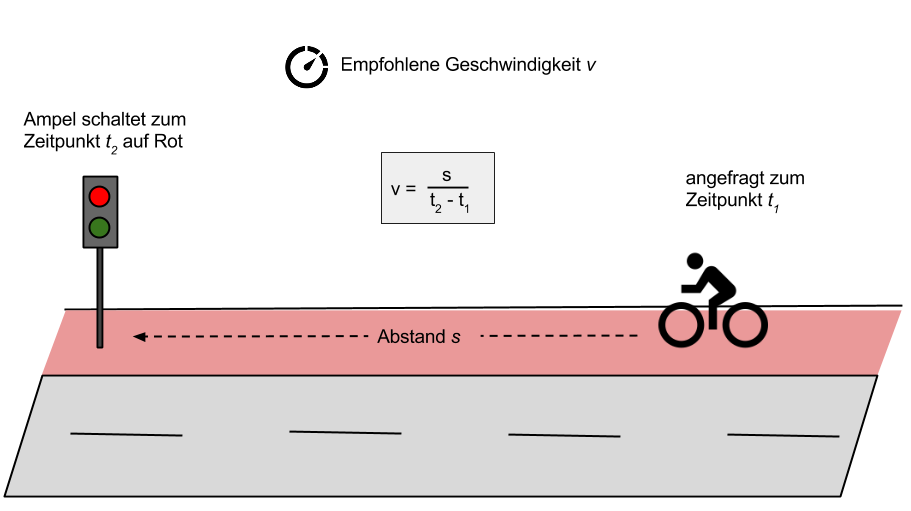
\includegraphics[width=1\textwidth]{vst}     
    \caption[Berechnung Progressionsgeschwindigkeit]{Veranschaulichung der Berechnung}
    \label{fig:vst}
\end{figure}
Um die ensprechende \gls{LSA} während der Grünphase zu passieren, muss letztendlich die empfohlene Geschwindigkeit $v$ eingehalten werden.
